\documentclass[a4paper,14pt]{article} 
\usepackage{lscape}
%%% Страница
\usepackage{extsizes} % Возможность сделать 14-й шрифт
\usepackage{geometry} % Простой способ задавать поля
        \geometry{top=25mm}
        \geometry{bottom=30mm}
        \geometry{left=30mm}
        \geometry{right=20mm}
 %

\usepackage[T1,T2A]{fontenc}
\usepackage[utf8]{inputenc}
\usepackage[english,russian]{babel}
\usepackage{amssymb,amsmath}
\usepackage{float}
\usepackage[unicode, pdftex]{hyperref}
\usepackage[europeanresistors,americaninductors]{circuitikz}
\usetikzlibrary{calc}
\usepackage[T1,T2A]{fontenc}
\usepackage[utf8]{inputenc}

\usepackage{amssymb,amsmath}
\usepackage{float}
\usepackage[unicode, pdftex]{hyperref}
\usepackage{booktabs}
\usepackage{multirow}

\usepackage{tikz}
\usepackage{rotating}
%\usepackage[landscape]{geometry}
\usepackage{graphicx}
\graphicspath{{pictures/}}
\DeclareGraphicsExtensions{.pdf,.png,.jpg}
\usepackage{pgfplots}
\usepackage{wrapfig}
\usepackage{rotating}
\usepackage{lipsum}
\usepackage{nccmath}
\usepackage{caption}
\usepackage{siunitx}
%\usepackage[american,cuteinductors,smartlabels]{circuitikz}
%\usepackage[backend=biber]{biblatex}

\usepackage[]{hyperref}
\ctikzset{bipoles/thickness=1}
\ctikzset{bipoles/length=0.8cm}
\ctikzset{bipoles/diode/height=.375}
\ctikzset{bipoles/diode/width=.3}
\ctikzset{tripoles/thyristor/height=.8}
%\ctikzset{tripoles/thyristor/width=1}
\ctikzset{tripoles/thyristor/width=0.8}
\ctikzset{bipoles/vsourceam/height/.initial=.7}
\ctikzset{bipoles/vsourceam/width/.initial=.7}
\tikzstyle{every node}=[font=\small]
\tikzstyle{every path}=[line width=0.8pt,line cap=round,line join=round]

\ctikzset{resistor = european}
\ctikzset{inductor = american}
\ctikzset{tripoles/thyristor/height=0.55}
\ctikzset{tripoles/thyristor/height 2=0.4}
%\ctikzset{tripoles/thyristor/width=0.35} 
\ctikzset{tripoles/thyristor/diode width left=0.35}
\ctikzset{tripoles/thyristor/diode width right=0.35}

\ctikzset{bipoles/cuteindictor/coils/.initial=3}
\ctikzset{bipoles/americanindictor/coils/.initial=3}
\ctikzset{bipoles/cuteindictor/coils/.initial=3}
\ctikzset{bipoles/americanindictor/coils/.initial=3}
\hypersetup{
colorlinks=false,
}
\usepackage{textcomp}

\begin{document}
%METHODICAL INSTRUCTIONS FOR PERFORMING LABORATORY WORKS

\section{Study of three-phase autonomous voltage inverter}

\subsection{Objective}

Study of electromagnetic processes, common characteristics and energy characteristics of a three-phase autonomous voltage inverter (AVI).


\subsection{Description of the laboratory setup}

The laboratory setup includes the following modules:
“Frequency converter” /Преобразователь частоты/, “Load” /Нагрузка/, “Power module" /Модуль питания/, “Thyristor converter” /Тиристорный преобразователь/, “Measuring module" /Модуль измерительный/, “Multimeters” /Мультиметры/, “Power meter” /Измеритель мощности/, a two-channel oscilloscope.

The Frequency Converter module provides conversion of alternating voltage 220 V with a frequency of 50 Hz into three-phase voltage with adjustable voltage and frequency values.

The front panels of the “Frequency Converter” and “Load” modules are shown in Fig. 1,2 respectively. The Frequency Converter module (see Fig. 1) contains:

\begin{itemize}
\item frequency converter E2-MINI-SP5L;
\item power connectors for supplying single-phase input voltage $A$ and $N$ and removing output voltage $A1$, $B1$ and $C1$;
\item power connectors for rectified voltage $U_d$: “+” connector $X5$ and “—” connector $X6$;
\item potentiometer for setting the control signal $PR1$ for simultaneous regulation of the frequency and output voltage;
\item button $SB1$ “Reset”/Сброс/ to reset the error after the protection has been triggered;
\item switch $SA1$, changing the phase sequence (direction of rotation);
\item frequency meter for measuring the frequency at the output of the AVI;
\item LEDs signaling power supply, normal operation and protection activation;
\item voltage (ДН) and current (ДТ) sensor for oscillography and measurements of voltages and currents in the circuit.
\end{itemize}

\begin{figure}[!ht]
\centering
\begin{minipage}[c]{0.4\textwidth}
\centering
    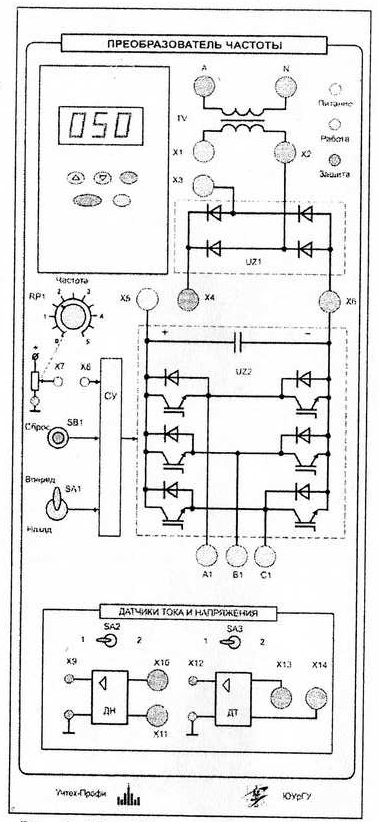
\includegraphics[width=2.5in]{lab7_fig1}
    \caption{Frequency converter}
    \label{fig:fc}
\end{minipage}
\noindent
\begin{minipage}[c]{0.4\textwidth}
\centering
    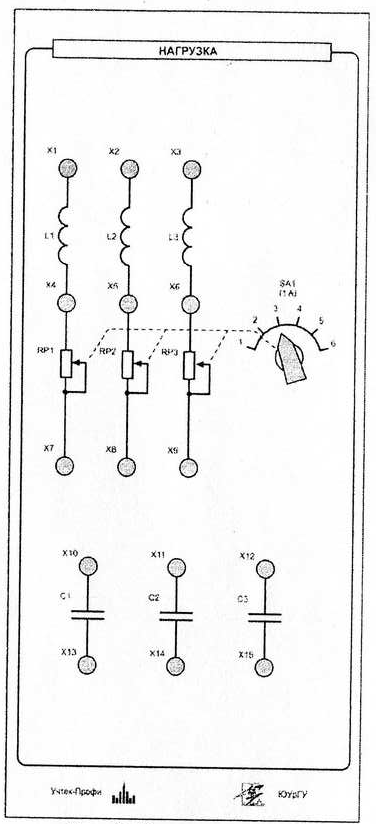
\includegraphics[width=2.5in]{lab7_fig2}
    \caption{Load}
    \label{fig:load}
\end{minipage}

\end{figure}

The module is powered from the AC mains through an isolation transformer $TV$, which provides potential isolation from the mains.

The Frequency Converter module consists of two units (see Fig. \ref{fig:fc}). The first unit of the frequency converter (FC) is an uncontrolled diode rectifier ($UZ1$), made using a single-phase bridge circuit. The second unit is a three-phase AVI made on IGBT transistors ($UZ2$). A capacitive filter is enabled at the $UZ2$ input.

In this work, we study the second unit - a three-phase autonomous voltage inverter.

The Frequency Converter module contains current (ДТ) and voltage (ДН) sensors, which are used for oscillography and measurement of voltages and currents in the circuit. Voltage signals are supplied to connectors $X10$ and $X11$, and current signals are supplied to connectors $X13$ and $X14$. Connectors $X9$, $X12$ and the common wire “$\perp$” are used to connect the output circuits ДТ and ДН to the oscilloscope or the input/output module.
Voltage sensor conversion coefficient $k_v = 40 V/V$, current sensor conversion coefficient $k_c = 0.25 A/V$. The actual voltage and current values are determined by multiplying the values measured using an oscilloscope by the corresponding sensor factor.

Using toggle switches $SA2$ and $SA3$ of the “Frequency Converter” module, the bandwidth of the sensors is changed, which allows you to observe either the PWM signal (position “2”) or its first harmonic (position “1”) on the screen of an oscilloscope or computer.

The “Frequency Converter” module is powered through sockets $A$ and $N$ of the three-phase alternating voltage source through the $QF2$ circuit breaker located in the power module.

The “Load” module (see Fig. \ref{fig:load}), containing reactors ($L1$ -- $L3$), resistors ($RP1$ -- $RP2$) and capacitors ($C1$ -- $S2$) is used as an AVI load.

In the “Load” module, only the active phase resistances ($RP1$ -- $RPЗ$) are regulated, and the reactive elements remain unchanged.
Regulation is made by switch $SA1$. The resistor values corresponding to the switch positions are given in table \ref{table:resistors}.

\begin{table}[!ht]

\begin{tabular}{l|c|c|c|c|c|c}

Switch position $SA1$ &1*& 2& 3& 4& 5& 6\\
\midrule
Load Resistance (Ohm) &100 &200 &400 &600 & 1000 & 1600
\end{tabular}
   \caption{}
    \label{table:resistors}
\end{table}

Note: “*” marks prohibited switch positions. The inductances ($L1$ -- $L3$) are $80 mH$, and the capacitances ($C1$ -- $C2$) are $10 \mu F$.

To obtain a three-phase active-inductive load, it is necessary to install jumpers between sockets $X7$ -- $X8$ and $X8$ -- $X9$ (zero load point).

\subsection{The procedure for turning the installation on and off}

\begin{enumerate}
\item Assemble an experimental scheme for performing laboratory work.
\item In the “Frequency Converter” module, set toggle switch $SA1$ (“Rotation direction”) to the middle position, frequency setting potentiometer $RP1$ to the zero position.
\item Set switch $SA1$ on the “Load” module to the position of maximum resistance (far right position).
\item Turn on the machine $QF1$ of the “power module of the stand”, turn on the machine $QF2$ of the “power module”.
\item Turn on the “Power” toggle switch of the “Power Meter” module.
\item In the “Frequency Converter” module, switch toggle switch SA1 to the upper position. The “Operation” LED will light up.
\item Use potentiometer $RP1$ to set the required frequency $f$ and the corresponding load voltage. In this case, the law $U_{l\;lin}/f = const$ is satisfied.
\item Set switch $SA1$ to the required resistance on the “Load” module.
\end{enumerate}

Shutdown procedure: turn off the $SA1$ toggle switch of the “Frequency Converter” module, and then the “Power” toggle switch of the “Power Meter” module, turn off the $QF2$ “Power Module” circuit breaker.

\subsection{Assignment and guidelines}

\begin{enumerate}
\item Preliminary homework:
\begin{enumerate}
\item study the topic of the course: “Autonomous voltage inverters”, “Energy indicators of rectifiers”, the content of this work and be ready to answer all test questions;
\item calculate the modulation coefficient $\mu$ for a given option. It is recommended to determine the modulation depth from the relation
\begin{equation}
\mu = \frac{U_{lin\;m}}{U_d} = \frac{f}{f_{max}}
\end{equation}
where $U_{lin\;m}$ is the amplitude value of the line-line voltage at the output of the AVI;

$U_d$ -- constant voltage at the input of the AVI;

$f$, $f_{max}$ are the specified and maximum frequency at the output of the AVI, respectively;

\item calculate for a given option the highest effective values of the first harmonic of line $U_{L\:lin(1)max}$ and phase $U_{L\:ph(1)max}$ voltages on the load for different modulation methods:

\begin{itemize}
\item[-] when generating average voltages at the terminals relative to the midpoint of the power source

\begin{equation}
U_{L\:lin(1)max} = \frac{\sqrt{3}\cdot U_d}{2\sqrt{2}}, \;\; U_{L\:ph(1)max} = \frac{U_d}{2\sqrt{2}}
\end{equation}

\item[-] when generating phase voltages using a space vector
\begin{equation}
U_{L\:lin(1)max} = \frac{U_d}{\sqrt{2}}, \;\; U_{L\:ph(1)max} = \frac{U_d}{\sqrt{6}}
\end{equation}

\end{itemize}
\item calculate the RMS-values of the first harmonic of line-line $U_{L\:lin(1)}$ and phase $U_{L\:ph(1)}$ voltages on the load for different modulation methods at a given frequency $f$ and the calculated modulation coefficient $\mu$:

\begin{equation}
U_{L\:lin(1)} = \mu U_{L\:lin(1)max},  \;\; U_{L\:ph(1)} = \mu U_{L\:ph(1)max}  
\end{equation}

\end{enumerate}


\item Experimental study of three-phase AVI:

\begin{enumerate}
\item assemble a circuit for studying a three-phase AIN when operating on an active-inductive load in accordance with Fig. 3. Additional jumpers and measuring instruments connected to the circuit are shown with a dashed line.

In table 2 shows measuring instruments, and table. 3 current and voltage sensors used in laboratory work, in accordance with the accepted designations on the circuit diagram (see Fig. 3).
table 2

\begin{table}[!ht]
\begin{tabular}{p{0.35\textwidth}p{0.15\textwidth}p{0.25\textwidth}p{0.25\textwidth}}
\toprule
Measured quantities& Device designation& Measurement limit & Device location (module name)\\
\midrule
Direct voltage at the input of the AVI $U_d$& $PV1$ & $=1000V$ &Multimeters\\
\midrule
Direct current at the AVI input $I_d$       & $PA1$ & $-$     & Measuring module\\
\midrule
RMS-value of the first harmonic of the phase voltage $U_{L\:ph(1)}$ and phase current $I_{L\:ph(1)}$ at the output of the AVI& $PW1$ &  $U_{L\:ph(1)}\approx 300V;$ $I_{L\:ph(1)}\approx 2A$ & 
Power meter
\end{tabular}
\caption{}
\label{table:II}
\end{table}
Set the toggle switches $SA2$ and $SA3$ of the voltage (ДН1 -- ДН2) and current (ДТ1 -- ДТ2) sensors in the “Thyristor Converter” and “Frequency Converter” modules to position “2” (the filter is off). Set the required measurement limits on measuring instruments according to table. \ref{table:II};

%Fig. 3. Schematic diagram for studying an autonomous voltage inverter when operating on an active-inductive load

\item take oscillograms of the first harmonic of the phase voltage $u_{L\:ph(1)}$ and current $i_{L\:ph(1)}$ at the output of the AVI using an oscilloscope for a given load resistance $R_L$ and control frequency $f$. To do this, connect the oscilloscope to the ДТ2 current sensor
(channel $CH2$ -- socket $X12$, connect the oscilloscope corpus to socket “$\perp$” ДТ2) and voltage sensor ДН2 (channel $CH1$ -- socket $X9$). Perform the necessary operations specified in the order in which the installation was turned on. Use potentiometer $RP1$ in the “Frequency Converter” module to set the specified value of control frequency $f$, and switch $SA1$ in the “Load” module set the specified value of load resistance $R_L$.

\begin{table}[!ht]
\begin{tabular}{p{0.45\textwidth}p{0.15\textwidth}p{0.30\textwidth}}
\toprule
Measured signal& Device designation& Device location (module name)\\
\midrule
Instantaneous voltage value at the AVI input $u_d$ & ДН1 & Thyristor converter\\
\midrule
Instantaneous current value at the AVI input $i_d$ & ДТ1 & Thyristor converter\\
\midrule
Instantaneous value of phase voltage at the output of the AVI $u_{L\:ph}$ & ДН2 & Frequency converter \\
\midrule
Instantaneous value of the phase current at the output of the AVI $i_{L\:ph}$ & ДТ2 & Frequency converter 
\end{tabular}
\caption{}
\label{table:III}
\end{table}

First, look at the oscillograms with a wide bandwidth of the sensors (position “2” of the toggle switches $SA2$ and $SA3$ of the “Frequency Converter” module), and then, switching the toggle switches $SA2$ and $SA3$ of the sensors to position “1”, sketch the oscillograms of the first harmonics of the phase voltage $u_{L\:ph(1)}$ and current $i_{L\:ph(1)}$. 
Pay attention to the phase shift between them (angle $\varphi$), as well as to the change in phase shift when the control frequency $f$ changes. 
Don't forget to define the voltage, current and time scales taking into account the sensor coefficients;

\item take oscillograms of voltage ud and current id at the input of the AVI at the same values of load resistance $R_L$ and control frequency $f$. 
To do this, connect the oscilloscope to the current sensor ДТ1 (channel $CH2$ - socket $X18$, connect the oscilloscope body to socket “$\perp$” ДТ1) and the voltage sensor ДН1 (channel $CH1$ -- socket $X15$). 
Explain the pulsed nature of the current consumed by the AVI at the input;

\item remove the regulating characteristics %adjustment
 $U_{L\:ph(1)} = F(f), \mu = F(f)$ and energy characteristics $P_d = F(f), P_L = F(f), S_L = F(f),\cos\varphi_L = F(f), \eta_L = F(f)$ of an autonomous voltage inverter when regulated according to the law $U/f=const$ and a given value $R_L$. Change the frequency in the range of 10 -- 50 Hz. To increase the measurement accuracy by eliminating interference, connect the zero point of the “Load” module (socket $X7$) to ground (socket $N$ of the “Power module”).

Record the following values and enter them into the table. 4:

\begin{itemize}
\item $f$ -- frequency at the output of the AI;

\item $U_d,I_d$ - constant voltage and current at the input of the AI, respectively;

\item $U_{L\:ph(1)}, I_{L\:ph(1)}$ are the RMS-values of the first harmonic of the phase voltage and current at the output of the AVI, respectively;

\item $I_{L\:ph}, \cos\varphi_L$  -- phase power at the output of the AIN and $\cos\varphi$ converter, measured by the “Power Meter” module, respectively.
\end{itemize}

Output power
\begin{equation}
P_d = U_d\cdot I_d
\end{equation}

Active and full power at load
\begin{equation}
P_L = 3\cdot P_{L\:ph},\;\;\; S_L = 3\cdot U_{L\:ph}\cdot I_{L\:ph}
\end{equation}
 

Efficiency coefficient AIN
\begin{equation}
\eta_L = P_L/P_d
\end{equation}


Modulation factor
\begin{equation}
\mu = \frac{\sqrt{3}\sqrt{2}U_{L\:ph(1)}}{U_d}
\end{equation}



\item repeat experiment 2d with a different value of Rн specified by the teacher. Based on the data of experiments 2d,d, construct the dependences Unf(1)


\end{enumerate}
\end{enumerate}

f) remove the external Unf(1) = F and the energy characteristics of an autonomous voltage inverter at a given frequency value f. To do this, use potentiometer RP1 in the “Frequency Converter” module to set the set frequency value f (frequency according to the device) and change the load current Inf with switch SA1 in the “Load” module. Record the same values as in experiment 2d, as well as the value of Rн.
Enter the data into the table. 5;

g) repeat experiment 2e with a different value of f specified by the teacher. Based on the data of experiments 2 f, g, construct the dependences Unf


Turn off the SA1 toggle switch of the “Frequency Converter” module, the “Network” toggle switch of the “Power Meter” module, as well as the QF2 “Power Module” and QF1 “Bench Power Module” circuit breakers.
Contents of the report

The report should contain the following points:

a) name and purpose of the work;

6) electrical circuit diagrams for performing experiments;

c) the results of experimental studies and calculations based on them,
placed in the appropriate tables;

D) experimentally measured and constructed characteristics;

e) processed oscillograms;

©) comparison of experimental results and preliminary calculations;

g) conclusions from the work:

— Indicate which modulation method is used in the AIN;

— explain the influence of load current on the regulating characteristics of the AUV;

— explain the influence of control frequency and load current on energy
AIN indicators.

Control questions

12.What is the difference between a slave and an autonomous inverter?
13.What is the difference between an autonomous voltage inverter and an autonomous inverter?
current?
14.Why are reverse diodes turned on in voltage inverters?
15.Why is there a capacitor at the input of the AI?
16.How to change the output frequency of a stand-alone inverter?
17.What depends on the carrier frequency?
18. Show the contours of current flow in a three-phase AIN.
19.How is the shape and magnitude of the voltage in the AIN regulated?
20. Compare the methods of generating phase voltages in three-phase AIN according to
maximum achievable voltages and switching losses.
21. Which autonomous inverters are most promising in electric drives in
present time?
22. What is the type of external characteristic of AIN? What does the slope of the characteristic depend on?

23. How to remove an external characteristic?

24. What is the regulating (frequency) characteristic of an autonomous inverter?

25. What type and why does the regulating (frequency) characteristic of the AIN for an electric drive have?
26. How to remove the adjustment (frequency) characteristic?
27. What determines the non-sinusoidal coefficient of the load current curve?
28. How to determine the efficiency of an AIN?
29. The procedure for turning on and off the laboratory installation.

\end{document}
